\documentclass[12pt]{article}

\usepackage[utf8]{inputenc}
\usepackage{latexsym,amsfonts,amssymb,amsthm,amsmath}
\usepackage{tikz}
\usepackage{stanli}
\usetikzlibrary{shapes,calc,through,3d,patterns}
\usetikzlibrary{arrows.meta,decorations.pathreplacing,angles,quotes}
\usepackage{multicol}
\usepackage{geometry}
\usepackage{mathtools}
\usepackage{siunitx}
\usepackage{booktabs}

\setlength{\parindent}{0in}
\setlength{\oddsidemargin}{-0.25in}
\setlength{\textwidth}{7in}
\setlength{\textheight}{9.3in}
\setlength{\topmargin}{-1in}
\setlength{\headheight}{18pt}

\newcommand\blfootnote[1]{%
    \begingroup
    \renewcommand\thefootnote{}\footnote{#1}%
    \addtocounter{footnote}{-1}%
    \endgroup
}

\definecolor{darkred}{rgb}{0.6,0,0}

\newcommand{\bolddelta}{\boldsymbol\delta}
\newcommand{\boldxi}{\boldsymbol\xi}

\begin{document}

\noindent ME473 - Dynamic finite element analysis of structures\hfill EPFL\\
Stefano Burzio \hfill 2025\\
\vspace{0.3cm}

\hspace*{\fill}\textbf{\Large Problem set 4}\hspace*{\fill}

\hrulefill


\subsection*{Problem 1}
We consider the transient heat conduction problem on a circular aluminum plate, denoted by \(\Omega\), with a radius \(a = 10 \, \text{cm}\). The governing equation for the temperature distribution $T(x,y,t)$ is given by
\begin{equation*}
    \rho c \frac{\partial T}{\partial t} = \text{div} (k \nabla T) + f_0, \quad \text{in } \Omega, \quad t > 0,
\end{equation*}
where:
\begin{itemize}
    \item \(\rho = 2700 \, \text{kg/m}^3\) is the density of aluminum,
    \item \(c = 900 \, \text{J/kg} \cdot \text{K}\) is the specific heat capacity of aluminum,
    \item \(k = 205 \, \text{W/m} \cdot \text{K}\) is the thermal conductivity of aluminum,
    \item \(f_0 = 10^6 \, \text{W/m}^2\) is the uniform internal heat source.
\end{itemize}
The temperature satisfies the following conditions:
\begin{itemize}
    \item Boundary condition: \(T = 0\) on $\partial\Omega$, the boundary of \(\Omega\).
    \item Initial condition: \(T(x, y, 0) = 0\), for all \((x, y) \in \Omega\).
\end{itemize}
Due to the symmetry of the problem, the temperature distribution is approximated using four bilinear triangular elements on an angular sector of \(45^\circ\), as illustrated in the following diagram:
\begin{center}
    \begin{tikzpicture}
        % Draw the axes
        \def\a{3}
        % Draw the walls
        \fill[pattern=north west lines] (0,0) circle (\a+0.5);
        \fill[white] (0,0) circle (\a cm);
        % Coordinates
        \coordinate (x1) at (0,0);
        \coordinate (x2) at (\a/2,0);
        \coordinate (x3) at (\a,0);
        \coordinate (x4) at (45:\a/2);
        \coordinate (x5) at (22.5:\a);
        \coordinate (x6) at (45:\a);
        \draw[-latex, ultra thin] (-\a-1, 0) -- (\a+1, 0) node[right] {$x$};
        \draw[-latex, ultra thin] (0, -\a-1) -- (0, \a+1) node[above] {$y$};
        % Draw the circle 
        \draw[thick] (0,0) circle (\a cm);
        % Draw the nodes
        \fill (x1) circle (2pt) node[below right] {$\mathbf x_{1}$};
        \fill (x2) circle (2pt) node[below right] {$\mathbf x_{2}$};
        \fill (x3) circle (2pt) node[below right] {$\mathbf x_{3}$};
        \fill (x4) circle (2pt) node[above left] {$\mathbf x_{4}$};
        \fill (x5) circle (2pt) node[right] {$\mathbf x_{5}$};
        \fill (x6) circle (2pt) node[right] {$\mathbf x_{6}$};
        % Draw the elements 
        \draw[thick] (x3) -- (x1) -- (x6);
        \draw[thick] (x2) -- (x4);
        \draw[thick] (x4) -- (x5) -- (x6);
        \draw[thick] (x2) -- (x5) -- (x3);
        % Label the elements 
        \node at (22.5:\a/4+0.2) {${}^1\Omega$};
        \node at (22.5:3*\a/5) {${}^3\Omega$};
        \node at (8:4*\a/5) {${}^2\Omega$};
        \node at (37:4*\a/5) {${}^4\Omega$};
    \end{tikzpicture}
\end{center}
The spatial discretization of the weak form leads to the following semi-discrete system:
\begin{equation*}
    \mathbf M \dot{\mathbf q} + \mathbf K \mathbf q = \mathbf r,
\end{equation*}
where:
\begin{multicols}{2}
    \begin{itemize}
        \item $\mathbf q$ is the vector of nodal temperatures,
        \item $\mathbf M$ is the heat capacity matrix,
        \item $\mathbf K$ is the thermal conductivity matrix,
        \item $\mathbf r$ is the heat source vector.
    \end{itemize}
\end{multicols}

Write a \texttt{MATLAB} script to:
\begin{enumerate}
    \item compute the global thermal conductivity and heat capacity matrices,
    \item compute the heat source vector $\mathbf r$ corresponding to the internal heat source $f_0$,
    \item solve the time-dependent system for a time span of $20$ s,
    \item plot the temperature distribution over time.
\end{enumerate}
\textsc{Hint}: use the \texttt{MATLAB} built-in function \texttt{ode45} to compute the transient temperature evolution over time

\end{document}